%++++Rename chapter: 'The Blow-Up Method'++++++++

In order to apply the Blow-Up Method to the fold point at the origin, we focus on a neighbourhood $U$ around the fold point $(0,0)$. 
The neigbourhood $U$ is small enough, such that $g(x,y, \epsilon) \neq 0$ in $U$, and we can define sections in $U$, as follows:
\begin{align*}
&\Delta ^{in} = \{ (x, \rho^2), x \in I \} \\
&\Delta ^{out} = \{ (\rho, y), y \in \mathbf{R} \},
\end{align*}
where $I \subset \mathbf{R}$. Now $\Delta^{in}$ is transverse to $S^a$, while $\Delta^{out}$ is transverse to the fast flow. This enables us to monitor the incoming trajectories from the attracting branch of $S$ and the trajectories leaving $U$ in the direction of the fast flow.
Then a function $\pi : \Delta^{in} \to \Delta^{out}$ can be defined, called the transition map, which describes how the trajectories passing through $\Delta^{in}$ are mapped onto the outgoing flow in $\Delta^{out}$.  
The following theorem describes the behaviour of the flow under $\pi$.
% and a sketch of the proof will be given at the end of this section: ++++last statement not precise+++

\begin{theorem}[\citealp{krupa2001}] \label{transition map theorem}
Under the assumptions made in this section, there exists $ \epsilon_0 >0$ such that the following assertions hold for $\epsilon \in (0, \epsilon_0]$:\\
1. The manifold $S_\epsilon^a$ passes through $\Delta^{out}$ at a point $(\rho, h(\epsilon))$, where $h(\epsilon) = O(\epsilon^{2/3})$.\\
2. The transition map $\pi$ is a contraction with contraction rate $O(e^{-c/\epsilon})$, where $c$ is a positive constant.
\end{theorem}
This means that the trajectories that enter $U$ through $\Delta^{in}$, will be funneled into a smaller section of $\Delta^{out}$ and therefore we are guaranteed to observe the trajectories that enter through $\Delta^{in}$ in $\Delta^{out}$. Now we are in the position to describe the method of Blow-Up Transformations in the neighbourhood $U$.

\subsection{Coordinate Transformation and Charts} \label{sec:transform blowup}
We first need to transform the extended system (\ref{extended FS}) with respect to the time variable and the space variables. This coordinate transformation is called the Blow-Up Transformation because the degenerate fold point $(0,0)$ is regarded as a sphere of radius $r=0$. By rescaling the space variables with respect to different weights of $r$,
\begin{subequations}
    \begin{align}
        &x=\Bar{r}\Bar{x}  \label{sys: blow up trans x}\\
        &y=\Bar{r}^2\Bar{y} \label{sys: blow up trans y}\\ 
        &\epsilon=\bar{r}^3\bar{\epsilon} \label{sys: blow up trans z},
    \end{align}  
    \label{sys: blow up trans}
\end{subequations}
we find that we are able to carry out further analysis, as will follow.
%+++++ If time and space permit, an analysis of the space B and coordinate map would be good... p.291 krupa++++
%A reasonable question to consider is why do we note consider spherical polar coordinates. The reasoning behind this is because we are looking to maximise our computational efficiency so we will proceed in cartesian coordinates.
Instead of analysing the sphere in spherical polar coordinates, which might seem the most obvious choice of method,  the rest of this analysis is done using charts, described below (see \citet{needam} for the construction of charts on a sphere). This method turns out to be a more natural choice for this problem and maximises computational efficiency.
\begin{figure}[h!]
	\centering
	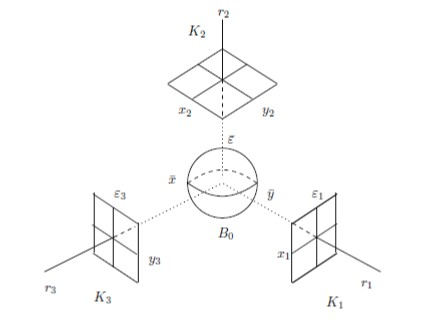
\includegraphics[height=5cm,width=7cm]{Images/charts-ball}
	\caption{Three charts mapping different sections of our blow up \citep{krupa2001}.}
	\label{fig:chartDiagram}
\end{figure}
In terms of the blown up fold point, a sphere denoted by $B$, charts are projections of regions of $B$ onto a two dimensional plane. 
We introduce three charts $ K_1,K_2,$ and $K_3 $. Chart $K_2$ is the two dimensional projection covering the upper half plane of $B$. However, as points on the equator of $B$ are approached on $K_1$, the point tends to infinity. These regions however, are of immense interest, since they are points of incoming and outgoing trajectories. As a consequence, charts $K_1$ and $K_3$ are introduced, covering the regions of interest on the equator of the fold point. 
%This is represented in Figure ++++++ (blow up figure)++
%The points that are relevant to the analysis of the dynamics are shown in Figure (+++insert figure 2.2 p,293+++++). (More description potentially)
The charts are defined by setting each of the variables of the extended system to $1$ in turn, giving $ \bar{y}=1, \ \bar{\epsilon}=1, \ \bar{x}=1 $. Substituting these into Equations (\ref{sys: blow up trans x}), (\ref{sys: blow up trans y}) and (\ref{sys: blow up trans z}) respectively gives, 
\begin{subequations} \label{ sys: K1K2K3}
	\begin{align}
	&x=r_1x_1, \ y=r_1^2, \ \epsilon=r_1^3\epsilon_1, \label{sys: K1}\\
	&x=r_2x_2, \ y=r_2^2y_2, \ \epsilon=r_2^3 \label{sys: K2}\\
	&x=r_3, \ y=r_3^2y_3, \ \epsilon=r_3^3\epsilon_3\label{sys:K3}
	\end{align}
\end{subequations}
where $ (x_i,r_i,\epsilon_i)\in\mathbf{R}^3 $ for $ i=1,2,3 $, and the equations correspond to the charts in numerical order \citep{krupa2001}. 
With this setup, we can consider the individual charts in turn, analyse the dynamics on the individual charts, and then join the gathered information into a global view on the dynamics in $U$.
We start with $K_2$,  because it holds the most information and the flow is the analysed more readily than in the other two charts. 
The remaining question is how the transition between the three charts and the connection to the global dynamics is made after finishing the individual analysis.
This is done via a coordinate change, derived by using Equations \ref{ sys: K1K2K3} and \ref{sys: blow up trans}, and the results are summarised in the following Lemma:
\begin{lemma} \label{coord. change}
Let $\kappa_{12}$ denote the change of coordinates from $K_1$ to $K_2$. Then $\kappa_{12}$ is given by \\
\begin{equation*}
x_2 = x_1 \epsilon_1^{-1/3},  y_2 = \epsilon_1^{-2/3}, r_2= r_1\epsilon_1^{1/3},
\end{equation*}
for $\epsilon_1 >0$,
and $\kappa_{12}^{-1}$ is given by
\begin{equation*}
x_1 = x_2y_2^{-1/2}, r_1 = r_2 y_2^{1/2}, \epsilon_1= y_2^{-3/2},
\end{equation*}
for $y_2>0$.
Let $\kappa_{23}$ denote the change of coordinates from $K_2$ to $K_3$. Then $\kappa_{23}$ is given by
\begin{equation*}
r_3 = r_2x_2, y_3= y_2x_2^{-2}, \epsilon_3 = x_2^{-3}, \label{eq:kappa23}
\end{equation*}
for $x_2>0,$
and $\kappa_{23}^{-1}$  is given by
\begin{equation*}
x_2 = \epsilon_3^{-1/3}, y_2 = y_3\epsilon_3^{-2/3}, r_2= r_3 \epsilon_3^{1/3},
\end{equation*}
for $\epsilon_3>0$.
\end{lemma}

Furthermore, transition maps $\Pi_i, i \in 1,2,3$  are defined in each section, describing how the trajectories coming in and out of each chart. These are combined in the final part of this section to give the proof of Theorem \ref{transition map theorem}, and to relate the results of the blow up method back to the original transition map $\pi$.
\newpage
\subsection{Dynamics in \texorpdfstring{$K_2$}{K2}} \label{sec: VDP K2}
\begin{figure}[h!]\centering
	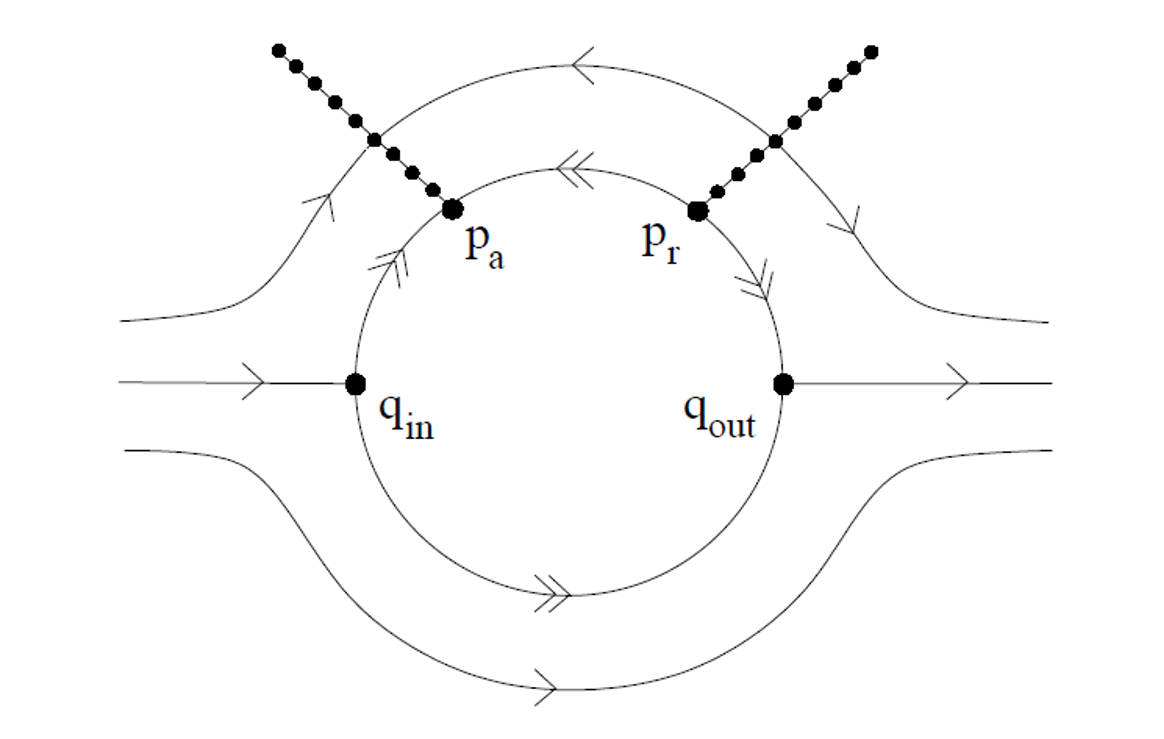
\includegraphics[height=4cm,width=6cm]{Images/Dynamics_in_Chart_2}
	\caption{Phase portrait for chart 2 \citep{krupa2001}.}
	\label{fig: chart 2 fig}
\end{figure}
To be able to consider chart $ K_2$, the transformation presented in Equation \ref{sys: K2} is applied to the extended system (\ref{extended FS}). Furthrmore,a time rescaling ($ t_2=r_2t $) is applied to desingularise the system. This results in:
\begin{equation}
	\begin{aligned}
		&\od{}{t}(r_2x_2)=r_2^2\od{x_2}{t}=-y_2+x_2^2-\dfrac{x_2^3r_2}{3},\\
		&r^3_2y'_2=r^3_2(-1+r_2x),\\
		&r'_2=0,
	\end{aligned}
\end{equation}
noting that $ \od{r}{t_2}=\od{t}{t_2}\od{r}{t}=\frac{1}{r_2}\od{r_2}{t} $ .  Now dividing through by $ r^2_2 $ and $ r^3_2 $ respectively for each equation and grouping $O(r_2)$ terms we get,
\begin{equation}
	\begin{aligned}
		&x'_2=x^2_2-y_2+O(r_2),\\
		&y'_2=-1+O(r_2),\\
		&r'_2=0.
	\end{aligned}
\end{equation}
Then, considering $r_2=0$ and neglecting the $O(r_2)$ terms results in,
\begin{equation} \label{Riccati}
	\begin{aligned}
		&x'_2=x^2_2-y_2,\\
		&y'_2=-1,\\
	\end{aligned}
\end{equation}
which are the well known Riccati equations- see \citet{Riccati}.
Some known results about the Riccati equations can be summarised as follows:


\begin{prop}[\citealp{krupa2001}]\label{Riccati Prop} 
The Riccatti equation (\ref{Riccati}) has the following properties:
\begin{enumerate}
\item Every orbit has a horizontal asymptote $y=y_r$, where $y_r$ depends on the orbit such that $x \to \infty$ as $y$ approaches $y_r$ from above.
\item There exists a unique orbit $\gamma_2$, which can be parameterized as $(x,s(x)), x \in \mathbf{R}$ and is asymptotic to the left branch of the parabola $x^2 - y = 0$, for $x \to - \infty$. The orbit $\gamma_2$ has a horizontal asymptote $y= - \Omega_0 <0$, such that $x \to \infty$ as $y$ approaches $-\Omega_0$ from above.
\item The function $s(x)$ has the asymptotic expansions
\begin{align*}
s(x) &= x^2 + \frac{1}{2x} + O\left( \frac{1}{x^4} \right), x \to -\infty,\\
s(x) &= -\Omega_0 + \frac{1}{x} + O\left( \frac{1}{x^3} \right), x \to \infty.
\end{align*}
\item All orbits to the right of $\gamma_2$  are backward asymptotic to the right branch of the parabola $x^2-y=0$.
\item All orbits to the left of $\gamma_2$ have a horizontal asymptote $y=y_l>y_r$, where $y_l$ depends on the orbit, such that $x \to -\infty$ as $y$ approaches $y_l$ from below.
\end{enumerate}
\end{prop}

The solutions to the Riccati equations, described in Proposition \ref{Riccati Prop}, are displayed in Figure. Note that the equation $x^2 - y=0$ is locally the critical manifold $S$ close to the fold point.%+++a bit wavy argument+++
The orbit $\gamma_2$, corresponds to the global trajectory $\gamma$, of the full system, which is the candidate trajectory connecting the slow flow on $S^a$ entering $U$ through $p_a$ to the fast fibres, exiting $U$ through $q_{out}$ - described by Figure \ref{fig: Ricatti Sol}. 
\begin{figure}[h!]\centering
	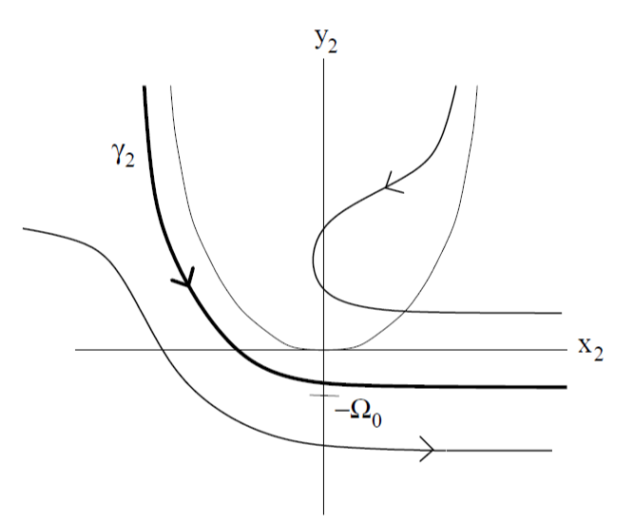
\includegraphics[height=6cm,width=6cm]{Images/Dynamics_in_K2}
	\caption{Ricatti solution for chart 2 \citep{krupa2001}.}
	\label{fig: Ricatti Sol}
\end{figure}
 
%(++++++refer back to figure  2.2 in krupa+++++++++)
This leads to the conclusion that if we can connect $\gamma_2$ to $p_a$  through $K_1$ and to $q_{out}$ through $K_3$, the global $\gamma$ can be constructed using Lemma \ref{coord. change}.
This motivates the analysis of $K_1$ and $K_3$.
In order to connect the dynamics on $K_2$ to that on the other charts, we need to define local inflow and outflow sections, similar to $\Delta^{in}$ and $\Delta^{out}$ in the full system.
Then we can follow trajectories that get mapped by $\Pi_2$, again analogous to $\pi$ in the full system, from a section $\Sigma^{in}_2$ to $\Sigma^{out}_2$.
The section are defined as follows. For $\delta>0$, we have:
\begin{align*}
\Sigma^{in}_2= \{ (x_2,y_2,r_2): y_2= \delta^{-2/3} \},\\
\Sigma^{out}_2 = \{ (x_2,y_2,r_2): x_2 = \delta^{-1/3} \}.
\end{align*}
Then the transition map $\Pi_2$ can be defined and the results are summarised as follows:
\begin{prop}[\citealp{krupa2001}]
The transition map $\Pi_2$ has the following properties:
\begin{enumerate}
\item
\begin{align*}
\Pi_2(q_0)= (\delta^{-1/3}, - \Omega_0 + \delta^{1/3} + O(\delta), 0)
\end{align*}
\item A neighbourhood of $q_0$ is mapped diffeomorphically onto a neighbourhood of $\Pi_2(q_0)$.
\end{enumerate}
\end{prop}
 
This is sufficient information to now consider the dynamics on $K_1$.

\subsection{Dynamics in \texorpdfstring{$K_1$}{K1}}\label{sec:dynamics-in-texorpdfstringk1k1} 
The coordinate transformation (\ref{sys: K1}) is applied to the extended system (\ref{extended FS}), 
\begin{align*}
\frac{d(r_1x_1)}{dt_1} \frac{dt_1}{dt} = -r_1^2 + r_1^2x_1^2 - \frac{1}{3}r_1^3x_1^3,\\
\frac{dr_1^2}{dt_1}\frac{dt_1}{dt}= 2r_1^2r_1' = r_1^3 \epsilon_1 (-1 +r_1 x_1),\\
\frac{d(r_1^3 \epsilon_1)}{dt_1}\frac{dt_1}{dt}= (3r_1^2\epsilon_1 + r_1^3 \epsilon_1') r_1 = 0.
\end{align*}
Dividing through by $\frac{dt_1}{dt}=r_1$ and replacing the expressions for $\epsilon_1'$ and $r_1'$ with their expressions in terms of the variables, results in the full system in terms of $K_1$. Note that the equation for $\epsilon'$ is found by rearranging the third equation above. 
\begin{align*}
x_1' &= -1 +x^2 + \frac{1}{2} x_1 \epsilon_1 + \left( - \frac{1}{2} \epsilon_1 x_1^2r_1 - \frac{1}{3} x_1^3 \right)\\
r_1' &= \frac{1}{2} r_1 \epsilon_1( -1 + r_1 x_1)\\
\epsilon_1' &= \frac{3}{2} \epsilon_1^2 ( 1- r_1x_1),
\end{align*}
and grouping terms in $r_1$ results in the standard form:
\begin{equation}
\begin{aligned} \label{K1systemfull}
x_1' &= -1 +x^2 + \frac{1}{2} x_1 \epsilon_1 +O(r_1)\\
r_1' &= \frac{1}{2} r_1 \epsilon_1( -1 + O(r_1))\\
\epsilon_1' &= \frac{3}{2} \epsilon_1^2 ( 1- O(r_1)).
\end{aligned}
\end{equation}

The system (\ref{K1systemfull}) has two invariant planes, that are somewhat equivalent to the notion of a nullcline. This tell us that the rate of change for our confidantes, $ r_1 $ and $ \epsilon_1 $ is constant for r$ _1=0 $ and $\epsilon_1=0$. If we substitute $r_1=0$ or $\epsilon_1=0$ into (\ref{K1systemfull}), the $r_1$ or $\epsilon_1$ equation respectively, are both zero, and there is only a two dimensional system left to consider. These two subspaces of (\ref{K1systemfull}) will be analysed below. Furthermore, the subspace where $r_1=0$ and $\epsilon_1=0$, is one dimensional, an invariant line, where the subspaces $r_1=0$ and $\epsilon_1=0$ cross.
The following analysis is displayed in Figure \ref{fig:k1chart}, illustrating the dynamics on $K_1$.
%\begin{figure}[h!]
%	\centering
%	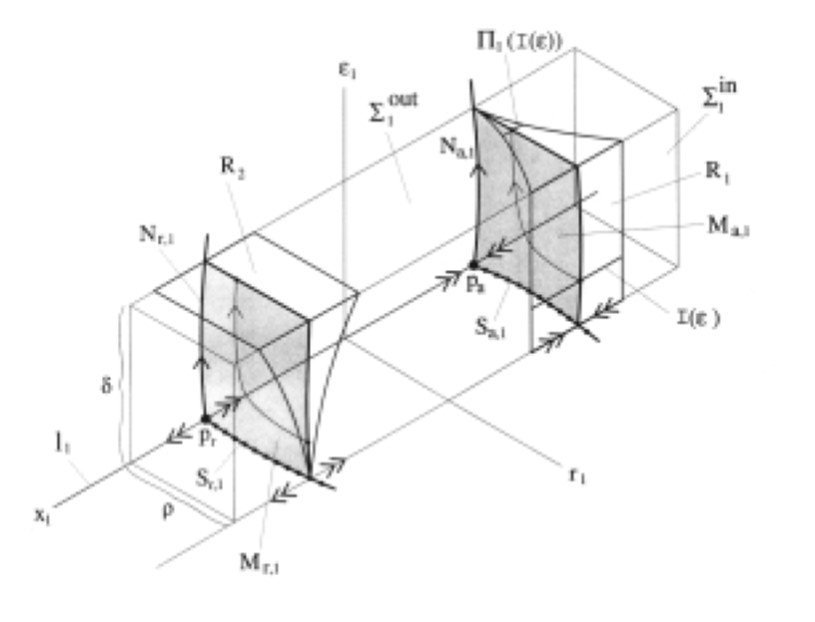
\includegraphics[width=7cm, height=7cm]{Images/K1Chart}
%	\caption{Dynamics in chart 1 \citep{krupa2001}
%	\label{fig:k1chart}
%\end{figure}
\begin{figure}[h!]
	\centering
	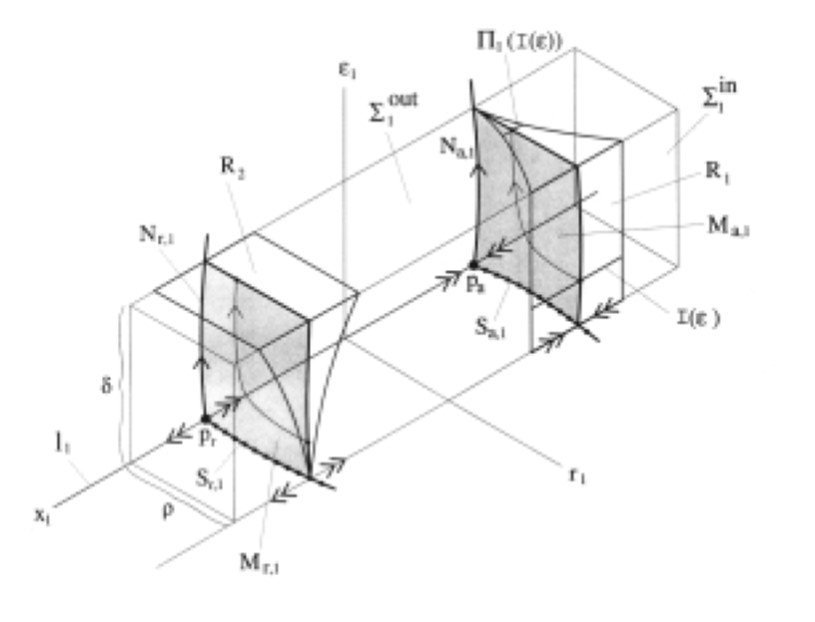
\includegraphics[height=7cm,width=7cm]{Images/K1Chart}
	\caption{Dynamics in chart 1 \citep{krupa2001}}
		\label{fig:k1chart}
\end{figure}\newpage


The invariant line, satisfying $r_1=0$ and $\epsilon_1=0$ is given by $l_1= -1 +x^2$. From this it is easily deduced that the two equilibrium points are where $l_1=0$, which is at $x=\pm1$. Therefore, the points $p_a$ and $p_r$ are defined as $p_a= (-1,0,0)$ and $p_r=(1,0,0)$. The flow on $l_1$ is attracted to $p^a$ and repelled by $p^r$, which is easily observed from the form $l_1$ takes or from a formal stability analysis of the one dimensional system. The eigenvalues of $l_1$ are found  by considering $l'_1 - \lambda = 2x - \lambda= 0 $ which gives that $\lambda = \pm 2$ at the respective equilibria. Then we expect the behaviour of the flow on the two invariant planes to be influenced by the two equilibria and the dynamics on $l_1$.
Consider the plane $\epsilon_1=0$. The system (Equation \ref{K1systemfull}) becomes
\begin{equation}
\begin{aligned} \label{epsilon0sys}
x_1' &= -1 +x_1^2 - \left( \frac{1}{3}r_1x_1^3 \right)\\
r_1' &= 0.
\end{aligned}
\end{equation}
This system has equilibria at $x= \pm1$, for $r_1=0$, as before, however, for each constant value of $r_1$, we get a different equilibrium of the system (\ref{epsilon0sys}). This forms a curve of equilibria, which can be recognised as $S^a_1$ connected to $p_a$ and $S^r_1$ connected to $p_r$, of the critical manifold, transformed into $K_1$ - this follows from the Implicit Function Theorem, see Figure \ref{fig: chart 2 fig}. The additional eigenvalue, corresponding to the $r_1$ equation, is $\lambda=0$. However, at each of the equilibria of this system, and specifically at $p_a$ and $p_r$ we have normal hyperbolicity, due to the coordinate transformation in $K_1$.% ++ go over this. +++
Next we consider the dynamics on the invariant plane $r_1=0$.
The system (Equation \ref{K1systemfull}) becomes: 
\begin{equation}
\begin{aligned}
x_1' &= -1 +x^2 + \frac{1}{2} x_1 \epsilon_1 \\
\epsilon_1' &= \frac{3}{2} \epsilon_1^2 .
\end{aligned}
\end{equation}
Again, $x= \pm 1$ are equilibria of the system, and an additional zero eigenvalue is gained due to the $\epsilon$ equation. It can be concluded that one dimensional centre manifolds exist, called $N_{a,1}$ and $N_{r,1}$, that are invariant, but not manifolds of equilibria like $S^a$ and $S^r$ in the $\epsilon=0$ plane. The dynamics on these manifolds are determined mainly by the value of $\epsilon$, since the change in the $\epsilon$ direction is much stronger than the change in the $x$ direction. Therefore, on $N_{a,1}$ and $N_{r,1}$ the flow moves in the $\epsilon$ direction with increasing epsilon.
In order to draw conclusions on the persistence of the dynamics in the full system, sections in the space are defined to monitor incoming and outgoing trajectories.
Firstly, let the region considered be such that
$D_1:= \{ (x_1,y_1,\epsilon_1): x_1 \in \mathbf{R}, 0, \leq r_1 \leq \rho, 0, \leq\epsilon_1 \leq \delta\}$.
Then the relevant sections for the candidate trajectory $\gamma$ are
\begin{align*}
\Sigma^{in}_1 := \{ (x_1,r_1, \epsilon_1) \in D_1 : r_1 = \rho \}, \\
\Sigma^{out}_1 := \{ (x_1,r_1, \epsilon_1) \in D_1 : \epsilon_1=\delta \}.
\end{align*}
Note that $\Sigma^{in}_1 = \Delta^{in}$ and $\Sigma^{out}_1=\Sigma^{in}_2$.
The aim is to find the connection between $p_a$ and $\gamma_2$ in $K_2$. In order to establish this connection, the trajectory $\gamma_2$ has to be mapped onto $K_1$ using Lemma \ref{coord. change}. Recall from Section \ref{sec: VDP K2} that the form of the candidate trajectory is of the form $(x_2, s(x_2))$.
Therefore, the trajectory $\gamma_1$ satisfies:
\begin{align*}
(x_1, 0, \epsilon_1) = \left(x_2 \left(x_2^2 + \frac{1}{2x_2} + O\left(\frac{1}{x_2^4} \right) \right)^{-1/2}, 0, \left(x_2^2 + \frac{1}{2x_2} + O\left(\frac{1}{x_2^4} \right)\right)^{-3/2} \right).
\end{align*}
Note that $s(x_2)$ as $x_2 \to - \infty$ is employed, since we consider the left continuation of $\gamma_2$.
Furthermore, as is intuitively clear from Figure \ref{fig: Ricatti Sol}, and can be shown by analysing the form of $\gamma_1$, the trajectory $\gamma_1$ converges to $p_a$ in backward time, which is exactly as expected.
This establishes the link between the slow flow on $S^a$ and the flow on $K_2$, if we consider the following proposition, which sums up the findings in $K_1$ and employs center manifold theory in order to establish persistence in the full system.
\begin{prop}[\citealp{krupa2001}]
For $\rho, \delta$ sufficiently small the following assertions hold for the system \ref{K1systemfull}:
\begin{enumerate}
\item There exists an attracting two-dimensional $C^k$- center manifold $M_{a,1}$ at $p_a$ which contains the line of equilibria $S_1^a$ and the center manifold $N_{a,1}$. In $D_1$ the manifold $M_{a,1}$ is given as a graph $x_1=h_a(r_1,\epsilon_1)$. The branch of $N_{a,1}$ in $r_1=0, \epsilon_1>0$ is unique.
\item There exists a repelling two-dimensional $C^k$- center manifold $M_{r,1}$ at $p_r$ which contains the line of equilibria $S_1^r$ and the center manifold $N_{r,1}$. In $D_1$ the manifold $M_{r,1}$ is given as a graph $x_1=h_r(r_1,\epsilon_1)$. The branch of $N_{r,1}$ in $r_1=0, \epsilon_1>0$ is not unique.
\item There exists a stable invariant foliation $F^s$ which base $M_{a,1}$ and one-dimensional fibres. For any $c>-2$ there exists a choice of positive $\rho$ and $\delta$ such that the contraction along $F^s$ during a time interval $[0,T]$ is stronger than $e^{cT}$.
\item There exists an unstable invariant foliation $F^u$ which base $M_{r,1}$ and one-dimensional fibres. For any $c>-2$ there exists a choice of positive $\rho$ and $\delta$ such that the expansion along $F^u$ during a time interval $[0,T]$ is stronger than $e^{cT}$.
\item The unique branch $N_{a,1}$ in $r_1=0, \epsilon_1>0$ is equal to $\gamma_1:= \kappa^{-1}_{12}(\gamma_2)$ wherever $\kappa^{-1}_{12}(\gamma_2)$ is defined, i.e. along the part of $\gamma_2$ corresponding to $y_2>0$.
\end{enumerate}
\end{prop}
 
In order to find the lower bound on the contraction rate along $F^s$, the transition time $T$  has to be found, i.e. the time the trajectory takes to travel from a point $p= (x_1, \rho, \epsilon_1)  \in \Sigma^{in}_1$ to a point in $\Pi_1(p)=( x_1, r_1, \delta) \in \Sigma^{out}_1$. This is done by integrating the $\epsilon$ equation of system (\ref{K1systemfull}), which is a separable ODE with respect to $t_1$.
This then results in 
\begin{align*}
T= \frac{2}{3} \left(\frac{1}{\epsilon_1} - \frac{1}{\delta} \right) \left( 1 + O(\rho) \right),
\end{align*}
where $r_1= \rho \in p$. 
Therefore, a transition map $\Pi_1: \Sigma^{in}_1 \to \Sigma^{out}_1$ can be defined for small enough parameter values of $\rho, \delta, \beta_1$. We are interested specifically in the transition around the center manifolds $M_{a,1}$ and $M_{r,1}$. The following subsections of $\Sigma^{in}_1 $ and $ \Sigma^{out}_1$ can be defined. Let $R_1= \{ (x_1, \rho, \epsilon_1) : |1+ x_1| \leq \beta_1 \}$, a rectangle in the intersection of the manifolds $M_{a,1}$ and  $\Sigma^{in}_1 $, and $R_2= \{ (x_1, r_1, \delta) : |1- x_1| \leq \beta_1 \}$, a rectangle in the intersection of the manifolds $M_{r,1}$ and  $\Sigma^{out}_1 $, with $\beta_1 >0$ sufficiently small. 
Furthermore, we can define line segments in these rectangles as $I_a(\overline{\epsilon}) \subset R_1$ and $I_r(\overline{r}) \subset R_2$, where $0 \leq \overline{\epsilon} \leq \delta$ and $0 \leq \overline{r} \leq \rho$.
Then for any $\overline{\epsilon}$, $\Pi_1$ maps the trajectory on a smaller region $\Pi_1 { I_a(\overline{\epsilon})} \in  \Sigma^{out}_1 $. This is called a contraction of the trajectories.
Considering Theorem \ref{transition map theorem}, which states the dependence of the contraction rate on $\epsilon$, the bounds on the contraction rate can be related to $\epsilon$, the parameter of the original system. Then using the $K_1$ rescaling of $\epsilon= \epsilon_1 r_1^3$, see Equation \ref{sys: K1},  the contraction rate for $\Pi_1 |I_r(\overline{r})$ is found by replacing $\epsilon_1$ by $\frac{\delta r^3_1}{\rho^3}$. 
Visual understanding of this analysis can be gained by considering Figure \ref{fig:k1chart}.
%++++ contraction in$ I_r$???+++++ 
The following proposition summarises the the findings for $\Pi_1$:
\begin{prop}[\citealp{krupa2001}]
For $\rho, \delta$ and $\beta_1$ sufficiently small, the transition map $\Pi_1: \Sigma^{in}_1 \to \Sigma^{out}_1$ defined by the flow of system \ref{K1systemfull} has the following properties:
\begin{enumerate}
\item $\Pi_1(R_1)$ is a wedge- like region in $\Sigma^{out}_1$. $\Pi_1^{-1}(R_2)$  is a wedge- like region in $\Sigma^{in}_1$.
\item More precisely, for fixed $c<2$, there exists a constant $K$ depending on the constants $c, \rho, \delta$ and $\beta_1$ such that:
\begin{enumerate}
\item for $\overline{\epsilon}\in (0, \delta] $ the map $\Pi_1 |I_a(\overline{\epsilon})$ is a contraction with contraction rate bounded by $Ke^{-\frac{2c}{3} \left(\frac{1}{\overline{\epsilon}} - \frac{1}{\delta} \right)}$.
\item for $\overline{r} \in (0, \rho] $ the map $\Pi_1 |I_r(\overline{r})$ is a contraction with coontraction rate bounded by $Ke^{-\frac{2c}{3} \left(\frac{\rho^3}{r_1^3 \delta} - \frac{1}{\delta} \right)}$.
\end{enumerate}
\end{enumerate}
\end{prop}

\subsection{Dynamics in \texorpdfstring{$K_3$}{K3}}\label{sec:dynamics-in-texorpdfstringk3k3}
The final chart to study the behaviour of is $K_3$. This chart covers the trajectory as it leaves the fold point at $q_{out}$. The other charts could not do this as $q_{out}$ is close to infinity in both $K_1$ and $K_3$ (cf. Figure \ref{fig:chartDiagram}). Similarly to $K_1$ and $K_2$, the system can be analysed using the blow-up transformation (\ref{sys:K3}).
\begin{subequations}
	\begin{align}
	\od{r_3}{t_3}&=r_3F(r_3,y_3,\epsilon_3) \\
	\od{y_3}{t_3}&=\epsilon_3(r_3-1)-2y_3F(r_3,y_3,\epsilon_3)\\
	\od{\epsilon_3}{t_3}&=-3\epsilon_3F(r_3,y_3,\epsilon_3)
	\end{align}
	\label{sys:K3blowup}
\end{subequations}
where $F(r_3,y_3,\epsilon_3)=\left(1-y_3-\frac{r_3}{3}\right)$. Note that as $\epsilon_3$ and $r_3$ appear as a factor in their respective derivatives, the planes $\epsilon_3=0$ and $r_3=0$ are invariant and, by extension, so is the $y_3$ axis.
The aim is to continue the special trajectory found in the other two charts and to find the transition map in and out of this chart. We will then be able to construct a phase portrait for the whole space by combining the dynamics in each chart. Linearising the system about $(0,0,0)=q_{out}$ gives 

\begin{align*}
\begin{pmatrix}\dot{r}_3\\\dot{y}_3\\\dot{\epsilon}_3\end{pmatrix}= \begin{pmatrix}
1 & 0 & 0 \\ 
0 & -2 & -1 \\ 
0 & 0 & -3
\end{pmatrix} \begin{pmatrix}
r_3 \\ 
y_3 \\ 
\epsilon_3
\end{pmatrix} 
\end{align*}
As the matrix is upper triangular, its eigenvalues are trivially  $\lbrace 1,-2,-3\rbrace$ with corresponding eigenvectors $\lbrace (1,0,0),(0,1,0),(0,1,1)\rbrace$. This presents an issue as there is additive resonance i.e. $\lambda_2-(\lambda_1+\lambda_3)=0$.  This means the Poincar\'e-Dulac theorem does not hold and the vector field is not linearisable, there is no smooth transformation between the nonlinear and linear flow. Despite this, progress can still be made as the form of the equations allow a near identity transformation and yields the lowest order approximation to the flow. %Note that $q_{out}$ is also  a hyperbolic equilibrium of the system.  +++Mention $\bar{M}_a$, the locally invariant perturbation of the center manifold $M_a$? Passes near the delicate equilibrium point $q_{out}$ so behaviour very much depends on how we pass this point. +++\\
The special orbit, $\gamma_2$, can be mapped into this chart using the change of coordinates $\kappa_{23}$ of Equation \ref{eq:kappa23}.
$$\gamma_3=\kappa_{23}(\gamma_2)$$
In fact, $\gamma_3$ lies in the plane $r_3=0$ and converges to $q_{out}$ as $\epsilon \to 0$. To find the flow in a neighbourhood of $q_{out}$ we use sections similar to those introduced in $K_2$.

\begin{align*} \Sigma_3^{in} =\lbrace(r_3,y_3,\epsilon_3) &: r_3\in[0,\rho], y_3 \in [-\beta_3,\beta_3], \epsilon_3=\delta\rbrace,\\
\Sigma_3^{out} =\lbrace(r_3,y_3,\epsilon_3) &: r_3=\rho, y_3 \in [-\beta_3,\beta_3], \epsilon_3\in[0,\delta]\rbrace
\end{align*}

We now wish to find the transition map $\Pi_3$ between these two charts. That is, given that the trajectory enters somewhere in $\Sigma_3^{in}$, how will it behave until it reaches $\Sigma_3^{out}$? To do this, the system \ref{sys:K3blowup} will be studied after some simplification. The system is in fact equivalent to the Riccati equation. Observe that $F(r_3,y_3,\epsilon_3)\big|_{q_{out}} = 1-y_3 + O(r_3)\big|_{q_{out}} \approx 1 $. Thus dividing (\ref{sys:K3blowup}) through by $F$ yields
\begin{subequations}
	\begin{align}
	\dot{r}_3&=r_3\\
	\dot{y}_3&=-2y_3 - \frac{\epsilon_3}{1-y_3}+r_3\epsilon_3 G(r_3,y_3,\epsilon_3)\\
	\dot{\epsilon}_3 &= -3\epsilon_3
	\end{align}
	\label{eq:K3ricc}
\end{subequations}

In the invariant plane $r_3=0$, the system becomes the Riccati equation (cf. (\ref{Riccati})) transformed into the chart $K_3$ and with a rescaling of time.
\begin{align*}
y'_3 &= -2y_3-\frac{\epsilon_3}{1-y_3}\\
\epsilon'_3 &= -3\epsilon_3
\end{align*}
This system has eigenvalues $\lbrace -2,-3\rbrace$ and the issue of additive resonance has been avoided so we are able to linearise the system using a near-identity transformation. This transformation allows the elimination of awkward higher order terms (in this case, $\frac{1}{1-y_3}$). Let
$$y_3=\psi(\tilde{y}_3,\epsilon_3)=\tilde{y}_3+O(\tilde{y}_3\epsilon_3).$$
Let $\tilde{\psi}$ denote the inverse transformation and both be $C^k$ functions. The system (\ref{eq:K3ricc}) can now be linearised and the following proposition gives the transition map.

\begin{prop}[\citealt{krupa2001}]
	The transition map $\Pi_3$ for the transformed $K_3$ system (\ref{sys:K3blowup}) is
	$$ \Pi_s(r_3,y_3,\delta) = \begin{pmatrix}
	\rho \\ 
	\Pi_{32}(r_3,y_3,\delta) \\ 
	\left(\frac{r_3}{\rho}\right)^3\delta
	\end{pmatrix} $$ 
	where $$\Pi_{32}(r_3,y_3,\delta)=\left(\bar{\psi}(y_3,\delta)-\delta\right)\left(\frac{r_3}{\rho}\right)^2 + O(r^3_3\ln r_3)$$
\end{prop}
\begin{proof}
	We will use the near-identity transformation to find the passage time $T$ and thus the values of $r_3,y_3,\epsilon_3$ at this time. For brevity, the subscripts will be omitted for the remainder of this proof. Under the near-identity transformation, system (\ref{eq:K3ricc}) becomes
	\begin{subequations}
		\begin{align}
		\dot{r} &= r,\label{sys:K3riccNIr}\\
		\dot{\tilde{y}}&=-2\tilde{y}+\epsilon+r\epsilon H(r,\tilde{y},\epsilon)\label{sys:K3riccNIy}\\
		\dot{\epsilon} &= -3\epsilon
		\label{sys:K3riccNIeps}
		\end{align}
	\end{subequations}
	Let the subscript $i$ denote the value of a variable at its entry into the chart, and likewise $o$ for out. Then $(r_i,y_i,\epsilon_i)\in \Sigma^{in}$, and $(r_o,y_o,\epsilon_o)\in \Sigma^{out}$. Thus 
	$$\begin{array}{c c c}
	r(0)=r_i & &r(T)=r_o=\rho\\
	y(0)=y_i & &y(T)=y_o\\
	\epsilon(0)=\epsilon_i=\delta& & \epsilon(T)=\epsilon_o
	\end{array}
	$$
	We wish to construct an equation for the out variables $(T,\tilde{y}_o,\epsilon_o)$ in terms of the in variables $ (r_i,\tilde{y}_i) $, that is the transition map. The $r$ and $\epsilon$ equations are easily solved:
	\begin{align}
	r&=r_ie^t &&\epsilon=\delta e^{-3t}
	\end{align}
	Then using $r(T)=\rho$, 
	$$r(T)=\rho=r_ie^-t \implies T=\ln\left(\frac{\rho}{r_i}\right).$$
	
	For the equation in $y$, a little more work is required. We introduce a new coordinate $z$ as follows, $\tilde{y}=e^{-2t}(\tilde{y}_i-\delta+z)+\delta  e^{-3t}$. Upon first sight, this seems unlikely to be of any use. However, it turns out that this transformation is ideal as it allows many terms to be removed. First rearrange for $z$ and differentiate with respect to $t$.
	\begin{align*}
	&z=e^{2t} (\tilde{y}-\delta e^{-3t})-\tilde{y}_i+\delta\\
	&\od{z}{t}= 2e^{2t}\tilde{y}+e^{2t}\dot{\tilde{y}}+\delta e^{-t}
	\end{align*}
	Substitute $\dot{\tilde{y}}$ from Equation (\ref{sys:K3riccNIy}) and cancel terms. 
	\begin{align*}
	&=e^{2t}(-\epsilon+r\epsilon H(r,\tilde{y},\epsilon))+\delta e^{-t}\\
	&=-\epsilon e^{2t}+e^{2t}r\epsilon  H(r,\tilde{y},\epsilon) + \delta e^{-t}\\
	&=e^{2t}r\epsilon  H(r,\tilde{y},\epsilon)
	\end{align*}
	This final equality follows from the explicit solutions in $r$ and $\epsilon$ above. These equations also show that $r\epsilon e^{2t} = r_i\delta e^{-2t}e^{2t}$. Finally,
	$$\dot{z} = r_iH^z(\,r_i,\tilde{y}_i,t)$$
	where $H^z$ is the same as $H$ but under the transformation from $z$, i.e. $H^z(\,r_i,\tilde{y}_i,t) = \delta H(r_ie^t,e^{-2t}(\tilde{y}_i-\delta+z)+\delta e^{-3t}, \delta e^{-3t})$. This has not affected the expression for the passage time $T$. +++Uniform boundedness of H implies?+++ Hence $z(T)=r_iO(T)=O(r_i\ln (\frac{\rho}{r_i}))$
	Using the initial definition of $z$, we recover an expression for $\tilde{y}(T)$.
	\begin{align*}
	\tilde{y}(T)&=e^{-2T}\left(\tilde{y}_i-\delta+O\left(r_i\ln\left(\frac{\rho}{r_i}\right)\right)\right)+\delta e^{-3T}\\
	&=(\tilde{y}_i-\delta)e^{-2\ln\frac{\rho}{r_i}}+e^{-2\ln\frac{\rho}{r_i}}O\left(r_i\ln\frac{\rho}{r_i}\right)+\delta \frac{r_i^3}{\rho^3}\\
	&=(\tilde{y}_i-\delta)\frac{r_i^2}{\rho^2}+O\left(\frac{r_i^3}{\rho^2}\ln\frac{\rho}{r_i}\right)
	\end{align*}
	We now have an expression for each of the out variables in terms of the initial conditions, albeit under a near-identity transformation. All that remains is to undo this transformation using the inverse map $\tilde{\psi}$.
	
	+++Undo transformation, explain $r$ and $\epsilon$ coordinates in prop. ThenDONE!+++
\end{proof}

\subsection{The Full Solution}
The analysis of the three charts, discussed in the Sections \ref{sec: VDP K2}-\ref{sec:dynamics-in-texorpdfstringk3k3}, provided a descripition of the dynamics on each of the charts, as well as theory to conclude the persistence of the dynamics in the full system.
The special trajectory $\gamma$ has been traced through all charts and in chart 1 it has been linked to the slow flow of $S^a$, while in chart 3 the connection to the fast flow has been made. Therefore, the fold point is indeed a jump point, or transition point, which connects the slow and fast dynamic.
These transition points can also be seen in the case of singular canards, which are treated in the following section.
The remaining issue is the transition of this special trajectory through the charts in order to have a solution of the full system. 
This is equivalent to finding the transition map $\pi$ from Theorem \ref{transition map theorem}.
Let $\Pi: \Sigma^{in}_1 \to \Sigma^{out}_3$ be the full transition map of the Blow-Up Transformation. Then it satisfies
\begin{align*}
\Pi := \Pi_3 \circ \kappa_{23} \circ \Pi_2 \circ \kappa_{12} \circ \Pi_1,
\end{align*}
where $\kappa$ is the change of coordinates defined in Lemma \ref{coord. change} and $\Pi_1, \Pi_2, \Pi_3$ are the transition maps in each chart.
Finally, reversing the blow up transformation gives the full transition map $\pi$ and therefore there exists a trajectory $\gamma$ in the blow down vector field connecting slow and fast flow.
With this analysis at hand we are now able to describe the full dynamics of the Van der Pol system when $\epsilon>0$ by analysing the singular limit $\epsilon \to 0$. 

The full result is visualised in Figure \ref{fig: vdp flow diagram}.
\begin{figure}[h!]\centering
		\begin{subfigure}[t]{0.45\textwidth}
			\centering
			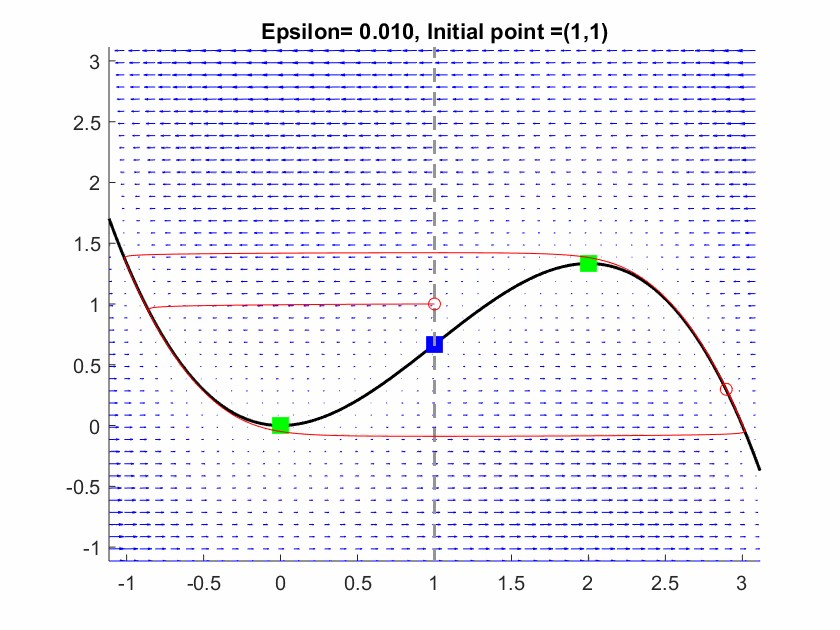
\includegraphics[width=.8\linewidth]{vdPe001-Moment-normal}
			\caption{The flow on the \vdp for a small $ \epsilon $.} \label{fig: vdp normal}
		\end{subfigure}
		\hfill
		\begin{subfigure}[t]{0.45\textwidth}
			\centering
			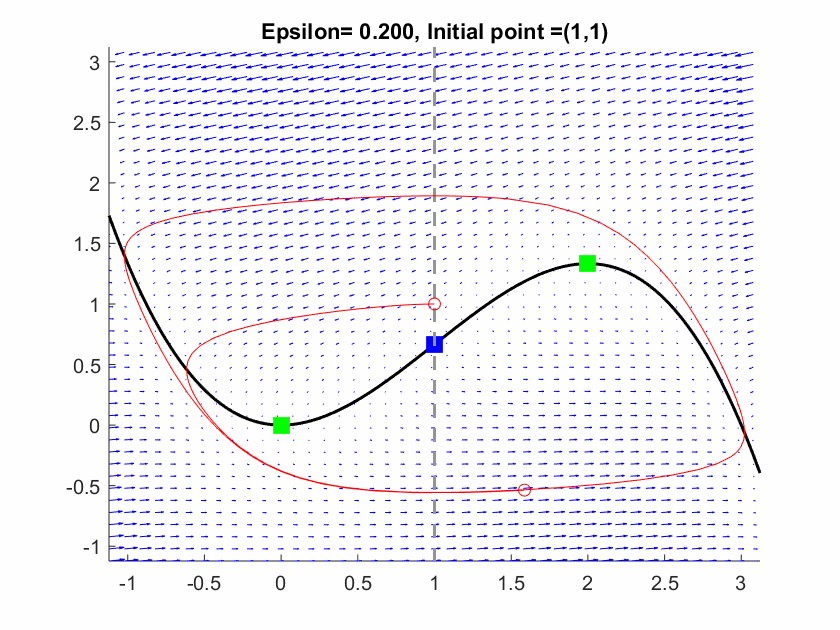
\includegraphics[width=.8\linewidth]{vdPe02-Moment-big-e}
			\caption{The flow on the \vdp for a larger $ \epsilon $.} \label{fig: vdp e.2}
		\end{subfigure}
		
%		\vspace{1cm}
%		\begin{subfigure}[t]{0.45\textwidth}
%			\centering
%			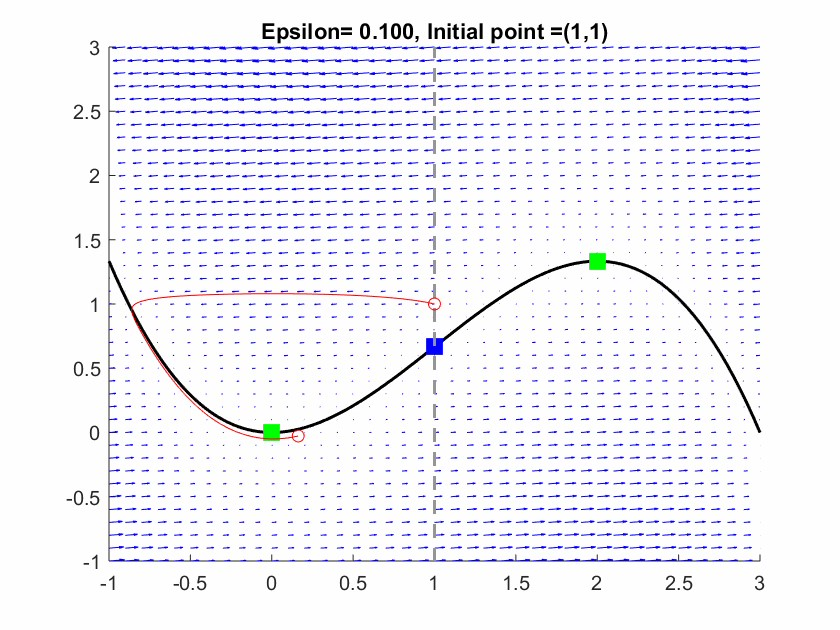
\includegraphics[width=.8\linewidth]{vdPhopf-Moment-3.jpg}
%			\caption{The flow as it intersects with the fold point.} \label{fig:timing3}
%		\end{subfigure}
%		\hfill
%		\begin{subfigure}[t]{0.45\textwidth}\centering
%			% just an empty subfigure to shift C below A
%			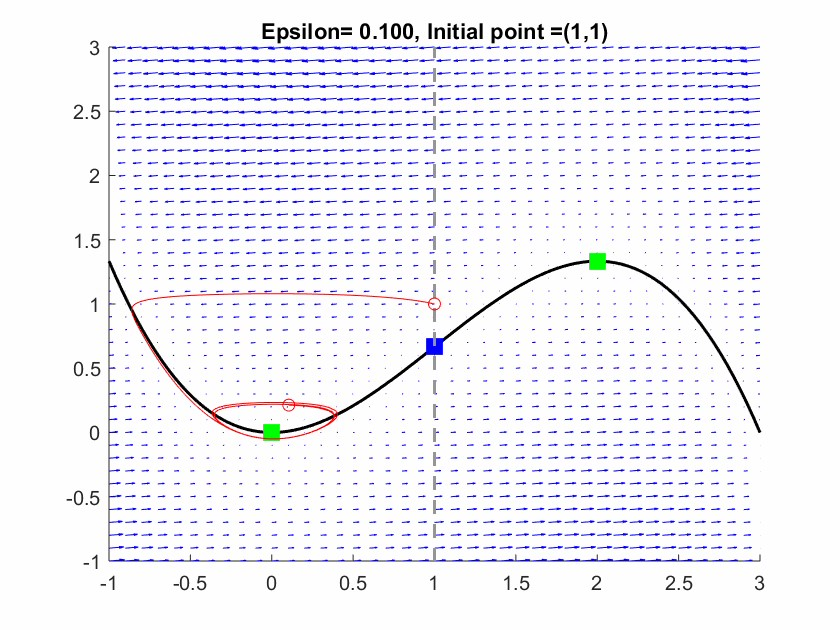
\includegraphics[width=.8\linewidth]{vdPhopf-Moment-4.jpg}
%			\caption{The Hopf bifurcation due to the canard point.}\label{fig:timing4}
%		\end{subfigure}
	\caption{Flow on the \vdp system.}
	\label{fig: vdp flow diagram e}
\end{figure}

























